\documentclass[oneside,b5paper,11pt]{article} %book class in 11 points
\usepackage{geometry} % Package re-sizing page for b5paper
\usepackage[hangul]{kotex} % Korean support
\usepackage{natbib} % cite style
\usepackage{paralist} % package for inline enumerate, i) ii)...

\usepackage{graphicx} % Allows including images

\usepackage{amsmath} % for math symbols
\usepackage{amssymb} % for math symbols

%\graphicspath{ {D:/_PlayGround/Github/2016_thesis/tex/images} }
\graphicspath{ {C:/My/Playground/Git/2016_Thesis/tex/images} }

\kscntformat{section}{}{} % 제 1.1절 -> 1.1
\renewcommand\thesection{\arabic{section}.} % 제 1.1절 -> 1.1
\renewcommand\thesubsection{\indent\arabic{section}.\arabic{subsection}.}


%%들여쓰기
\usepackage{indentfirst}
\setlength\parindent{2.0em}


\title{논문 연구 진행 보고}
\author{김동완}
\date{\today}

\begin{document}

%%%%%%%%%%
% Starting document.
%%%%%%%%%%


\maketitle

% Section
\section{전체 진행 계획}
\begin{enumerate}
	\item 가상 데이터 실험
	\begin{enumerate}
		\item 데이터 생성(연속형 설명변수, 이항 반응변수) \textbf{[완료]}
		\item Online Gradient Descent방법 실험 \textbf{[완료]}
		\item Assumed Density Filtering 방법 실험 \textbf{[완료]}
	\end{enumerate}

	\item 작은 규모의 실제 데이터 실험
	\begin{enumerate}
		\item 범주형 변수에 대한 Feature Hashing(murmurhash) \textbf{[완료]}
		\item Online Gradient Descent방법 실험 \textbf{[완료]}
		\item Assumed Density Filtering 방법 실험 \textbf{[완료]}
	\end{enumerate}
	
	\item 큰 규모의 실제 데이터 실험
	\begin{enumerate}
		\item Online Gradient Descent방법 실험
		\item Assumed Density Filtering 방법 실험
	\end{enumerate}

\end{enumerate}

 
 
% Section
\section{연구 개요}
 배치 처리가 어려울 정도로 건수가 많고, 범주의 수가 유동적인 수백 개의 범주형 변수를 갖는 데이터에 대한 온라인 베이지안 로지스틱 회귀분석 기법에 대한 연구



% Section
\section{지난 세션 진행 내용 개괄}

\subsection{개요}
 한개의 연속형 설명변수와 이항 반응 변수를 갖는 데이터를 모의로 3000건 생성하여 Online Gradient Descent 방법과 Assumed Density Filtering 방법으로 로지스틱 회귀 모형을 적합하고, 그 회귀 모수 값의 변화를 ML추정치와 비교
\subsection{결과}
 Gradient Descent 방법을 적용한 경우 Step size $\alpha$의 값에 따라 ML추정치로의 근사 속도가 달라짐, Assumed Density Filtering 방법을 적용한 경우 각 모수 분포의 초기 평균과 분산 값에 따라 근사 속도가 달라짐

 Gradient Descent의 경우 각 모수에 따른 최적의 Step size를 찾거나 iteration에 따라 이를 유동적으로 변화 시켜주는 방법이 필요한데, Assumed Density Filtering 방법의 경우 각 모수의 불확실성을 모수 분포의 분산으로 모델링 하여 Step size를 유동적으로 변화시키는 효과를 얻을 수 있음.
실험 결과에서도 이러한 효과가 반영되어 초기 적합 속도가 우수한 것을 확인 할 수 있었음.



% Section
\section{이번 세션 진행 내용}
\subsection{개요}
 대규모 데이터에 앞서의 방법론을 적용하기에 전에 우선 간단한 데이터를 이용하여 feature hashing방법으로 데이터를 가공한 후  Online Gradient Descent와 Assumed Density Filtering 방법으로 모형 적합을 수행하고, 그 결과를 ML추정치를 사용한 예측 결과와 비교하려 함.

 범주의 개수가 유동적이고 범주형 변수가 많이 포함된 데이터를 분석할 경우 dummy 변수의 갯수가 많아지고, 범주가 추가될 때 마다 다시 dummy 변수를 갱신하거나 모형 적합을 다시 수행해야는 문제가 발생한다. 이러한 문제에 대한 대응 방법으로 feature hashing(hashing trick, kernel trick) 을 사용.

 이 실험에서는 Kaggle\footnote{https://www.kaggle.com/c/titanic}에 공개된 891건의 데이터를 사용했고, 800건을 이용하여 모형 적합을 수행하고 나머지 91건에 대하여 MLE, OGD, ADF 방법의 정-예측률을 비교.

\subsection{데이터 설명}
\begin{itemize}
	\item Survived : 0, 1 \textbf{[반응 변수]}
	\item Pclass : 1, 2, 3
	\item Sex : male, female
	\item Age : 0.67 $\sim$ 80
	\item SibSp : 0, 1, ... , 7, 8
	\item Parch : 0, 1, 2, 3, 4, 5, 6
	\item Fare : 0 $\sim$ 512.3292
	\item Embarked : C, Q, S
\end{itemize}

\subsection{Feature hashing}
 다양한 hashing 방법 중 비교적 hash 충돌이 양호하다고 알려진 murmurhash 방법을 사용(R의 digest 패키지에서 제공)

 이 데이터의 경우 모든 변수를 범주형으로 취급하여 [변수명 + 값]에 hashing을 적용할 경우 350여 가지의 16진수가 생성되었고, 이 값을 512로 모듈러 연산하여 회귀 계수 벡터의 인덱스로 사용함\footnote{첨부 R code의 get\_mur\_x\_v3(df\_row) 함수}.
 

\subsection{3가지 방법을 이용한 결과 비교}
\begin{itemize}
	\item ML 추정치를 이용한 예측(dummy 변수 사용)
	\item Online Gradient Descent를 사용한 예측(feature hashing)
	\item Assumed Density Filtering을 사용한 예측(feature hashing)
\end{itemize}

위 세가지 방법을 사용하여 회귀 계수를 구하고 테스트 데이터 91건에 대한 예측을 수행한 후 예측률을 비교해봄.
 Online Gradient Descent의 경우 alpha값이 0.2 $\sim$ 0.3일때, Assumed Density Filtering의 경우 초기 분산 값이 2 $\sim$ 9 일때 가장 높은 예측률을 보였음.


 91건의 테스트 데이터에 대한 3가지 방법의 정-예측률을 비고하면 아래와 같은데, 온라인 예측의 특성상 ML추정치를 이용한 예측률에는 미치지 못했으나 큰 차이는 아니라고 할 수 있음.

\begin{table}[ht]
	\caption{예측률 비교 }
	\centering
	\begin{tabular}{c c c c}
	\hline\hline
	%\toprule
	\textbf{} & \textbf{MLE} & \textbf{OGD} & \textbf{ADF}\\
	\hline
	%\midrule
	  & 0.8427 & 0.8315 & 0.8315 \\
	\hline
	%\bottomrule
	\end{tabular}
\end{table}


 Online Gradient Descent와 Assumed Density Filtering의 반복 당 평균 log-loss를 비교하면 아래와 같음. 두 방법 모두 iteration이 증가할 수록 일정한 값으로 수렴함을 알 수 있음.

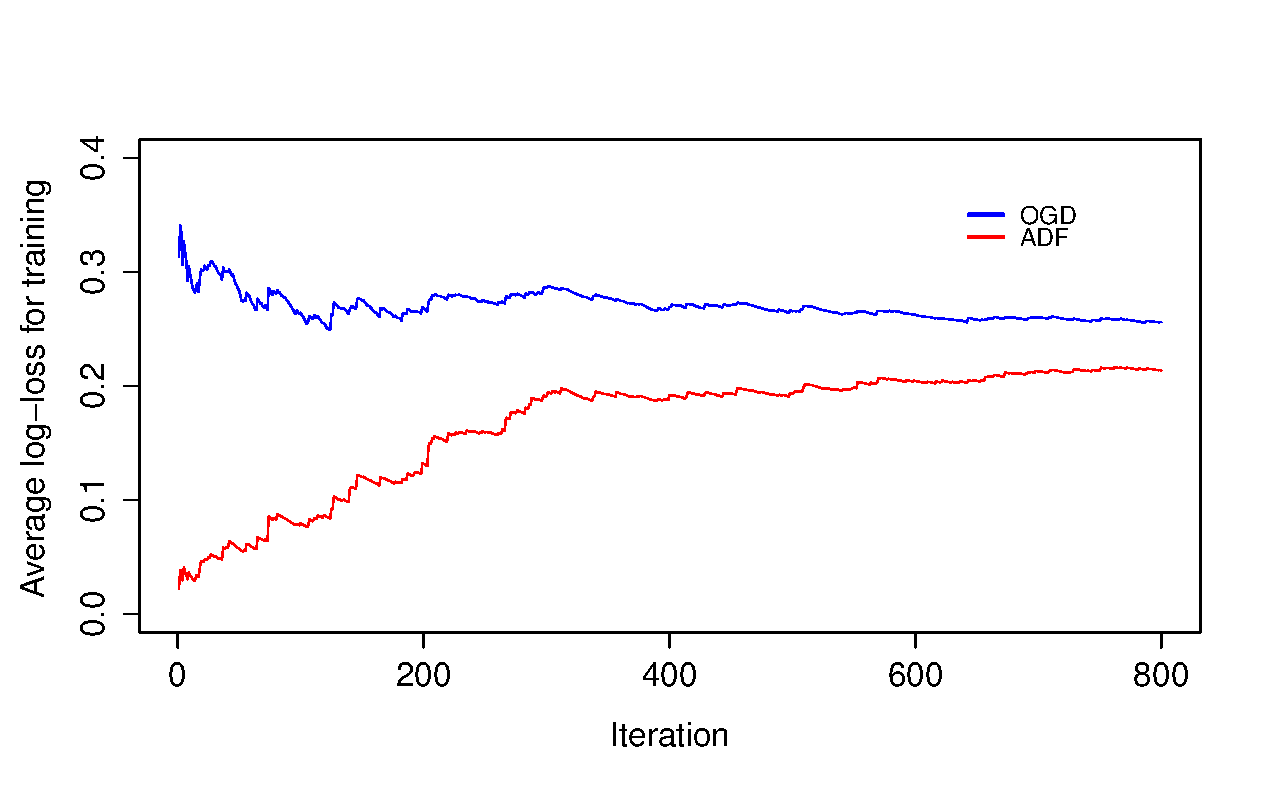
\includegraphics[scale=0.55]{titanic_ogd_adf.eps} %730 * 430

% Section
\section{다음 세션 진행 계획}
 앞서 titanic 데이터에서 구현한 feature hashing 방법을 동일하게 적용하여 4천 500만건 정도의 온라인 광고 데이터에 대해 OGD, ADF 두가지 방법을 실험하고 결과를 비교 분석 예정.











\end{document}